\documentclass[aspectratio=169,11pt]{beamer}

\usetheme{Madrid}
\usecolortheme{default}
\setbeamertemplate{navigation symbols}{}
\setbeamertemplate{footline}[frame number]

\usepackage{amsmath,amssymb}
\usepackage{graphicx}
\usepackage{tikz}
\usetikzlibrary{positioning,calc}
\usetikzlibrary{arrows.meta,decorations.pathmorphing}

\definecolor{RamRed}{RGB}{190,40,45}
\definecolor{RamBlue}{RGB}{30,90,180}
\definecolor{SoftGray}{RGB}{245,245,245}
\definecolor{DarkGray}{RGB}{70,70,70}
\definecolor{MapGreen}{RGB}{48,150,95}
\definecolor{MapGold}{RGB}{235,180,45}

\setbeamercolor{title}{fg=DarkGray}
\setbeamercolor{frametitle}{fg=white,bg=RamBlue}
\setbeamercolor{structure}{fg=RamBlue}

\tikzset{
  v/.style={circle,draw=black,fill=white,inner sep=1.8pt},
  edge/.style={draw=RamBlue,line width=1.25pt},
  topic/.style={draw=black!30,fill=SoftGray,rounded corners=5pt,inner sep=7pt,
    text width=5.8cm,minimum height=1.65cm,align=left},
}


\usepackage{booktabs}
\tikzset{dot/.style={circle,fill=black,inner sep=2pt}, lab/.style={circle,draw=black,fill=white,inner sep=2pt,minimum size=6mm,font=\small},selected/.style={draw=RamRed,line width=2pt}}

\newcommand{\Def}[2]{\begin{block}{#1}#2\end{block}}
\newcommand{\Thm}[2]{\begin{block}{#1}#2\end{block}}
\renewcommand{\Proof}[1]{\begin{block}{Proof}\normalsize #1\end{block}}
\newcommand{\Question}[1]{\begin{block}{Question}#1\end{block}}
\renewcommand{\Example}[1]{\begin{block}{Example}#1\end{block}}
\newcommand{\fall}[2]{#1^{\underline{#2}}}
\newcommand{\rise}[2]{#1^{\overline{#2}}}
\newcommand{\stir}[2]{\left\{\begin{matrix}#1\\#2\end{matrix}\right\}}
\newcommand{\cyc}[2]{\left[\begin{matrix}#1\\#2\end{matrix}\right]}
\newcommand{\eul}[2]{\left\langle\begin{matrix}#1\\#2\end{matrix}\right\rangle}
\newcommand{\coef}[2]{[#1^{#2}]}
\newcommand{\gap}{\par\medskip}

\title{Inclusion and Exclusion}
\author{Jeremy Quastel}\date{}\begin{document}
\begin{frame}[plain]\begin{center}{\Huge\bfseries Inclusion and Exclusion}\par\vspace{.25cm}{\Large Section 2.5}\par\vspace{.15cm}{\large Harris--Hirst--Mossinghoff, \emph{Combinatorics and Graph Theory}}\par\vspace{.1cm}\resizebox{!}{2.7cm}{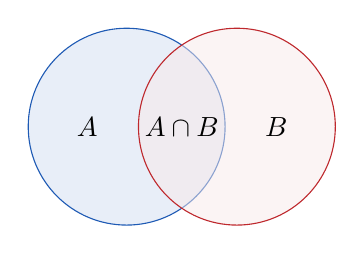
\begin{tikzpicture}\draw[RamBlue,fill=RamBlue!10](-.7,0)circle(1.25);\draw[RamRed,fill=RamRed!10,fill opacity=.5](.7,0)circle(1.25);\node at(-1.2,0){$A$};\node at(1.2,0){$B$};\node at(0,0){$A\cap B$};\end{tikzpicture}}\par\vspace{.25cm}Jeremy Quastel\end{center}\end{frame}
\begin{frame}[plain]\large \begin{center}{\Huge\bfseries Today\textquotesingle s lecture}\par\vspace{.5cm}\end{center}\begin{columns}[c,onlytextwidth]\begin{column}{.48\textwidth}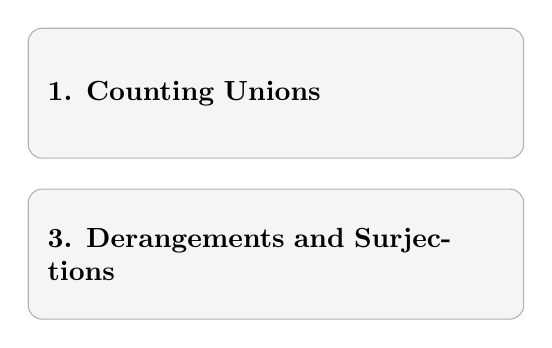
\begin{tikzpicture}\node[topic](a){\textbf{1. Counting Unions}};\node[topic,below=.38cm of a]{\textbf{3. Derangements and Surjections}};\end{tikzpicture}\end{column}\begin{column}{.48\textwidth}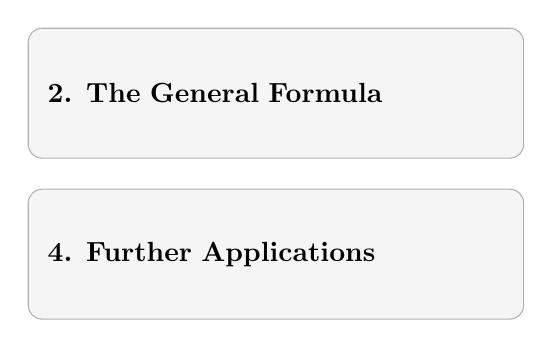
\begin{tikzpicture}\node[topic](a){\textbf{2. The General Formula}};\node[topic,below=.38cm of a]{\textbf{4. Further Applications}};\end{tikzpicture}\end{column}\end{columns}\end{frame}
\begin{frame}{Counting overlapping sets}
\large
\begin{center}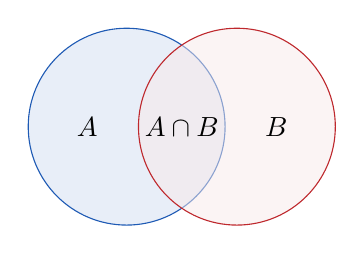
\begin{tikzpicture}\draw[RamBlue,fill=RamBlue!10](-.7,0)circle(1.25);\draw[RamRed,fill=RamRed!10,fill opacity=.5](.7,0)circle(1.25);\node at(-1.2,0){$A$};\node at(1.2,0){$B$};\node at(0,0){$A\cap B$};\end{tikzpicture}\end{center}
\[|A\cup B|=|A|+|B|-|A\cap B|.\]
\end{frame}
\begin{frame}{Three sets}
\large
\Thm{Formula}{\begin{align*}
|A\cup B\cup C|={}&|A|+|B|+|C|\\
&-|A\cap B|-|A\cap C|-|B\cap C|\\
&+|A\cap B\cap C|.
\end{align*}}
\gap Elements belonging to all three sets are added three times, subtracted three times, and finally added once.
\end{frame}
\begin{frame}{Inclusion and exclusion}
\large
\Thm{Principle of inclusion and exclusion}{For finite sets $A_1,\ldots,A_r$,
\[\left|\bigcup_{i=1}^r A_i\right|
=\sum_{\varnothing\ne I\subseteq[r]}(-1)^{|I|+1}
\left|\bigcap_{i\in I}A_i\right|.\]}
\gap Add single sets, subtract pairwise intersections, add triple intersections, and continue with alternating signs.
\end{frame}
\begin{frame}{Proof by following one element}
\large
\Proof{An element lying in exactly $t\geq1$ of the sets is counted
\[\binom t1-\binom t2+\cdots+(-1)^{t+1}\binom tt\]
times. Since $\sum_{j=0}^t(-1)^j\binom tj=0$, this alternating sum is $1$.\gap An element in none of the sets is never counted. Thus the formula counts the union exactly once.}
\end{frame}
\begin{frame}{Counting objects avoiding every bad property}
\large
\Thm{Complement form}{If all $A_i\subseteq U$, then
\[\left|U\setminus\bigcup_{i=1}^r A_i\right|
=\sum_{I\subseteq[r]}(-1)^{|I|}\left|\bigcap_{i\in I}A_i\right|,\]
where the intersection for $I=\varnothing$ means $U$.}
\gap Let $A_i$ describe a forbidden property.
\end{frame}
\begin{frame}{Integers divisible by $2$, $3$, or $5$}
\large
\Question{How many integers from $1$ to $100$ are divisible by at least one of $2,3,5$?}
\gap The individual counts are $50,33,20$. Pairwise intersections count multiples of $6,10,15$, and the triple intersection counts multiples of $30$.
\end{frame}
\begin{frame}{The divisibility calculation}
\large
\[50+33+20-16-10-6+3=74.\]
\gap Hence $100-74=26$ integers in the range are divisible by none of $2,3,5$.
\gap Intersections are counted using least common multiples; multiplying divisors works here because the original divisors are pairwise coprime.
\end{frame}
\begin{frame}{Derangements}
\large
\Def{Derangement}{A derangement is a permutation with no fixed point. Let $D_n$ be the number of derangements of $[n]$.}
\Example{For $n=3$, the derangements in one-line notation are $231$ and $312$. Thus $D_3=2$.}
\end{frame}
\begin{frame}{Derangements: identify the bad sets}
\large
Let $U$ be the set of all $n!$ permutations, and let
\[A_i=\{\pi:\pi(i)=i\}.\]
\gap If a specified set of $k$ positions is fixed, the remaining positions can be permuted in $(n-k)!$ ways.
\gap There are $\binom nk$ such sets of positions.
\end{frame}
\begin{frame}{The derangement formula}
\large
\Thm{Theorem}{\[D_n=\sum_{k=0}^n(-1)^k\binom nk(n-k)!
=n!\sum_{k=0}^n\frac{(-1)^k}{k!}.\]}
\Proof{Apply inclusion and exclusion to the sets of permutations fixing each position.}
\end{frame}
\begin{frame}{Small derangement numbers}
\large
\begin{center}\renewcommand{\arraystretch}{1.6}
\begin{tabular}{c|rrrrrrr}
$n$&0&1&2&3&4&5&6\\\hline
$D_n$&1&0&1&2&9&44&265
\end{tabular}\end{center}
\gap The empty permutation gives $D_0=1$.
\gap For example, $D_4=24-24+12-4+1=9$.
\end{frame}
\begin{frame}{A derangement recurrence}
\large
\Thm{Theorem}{For $n\geq2$,
\[D_n=(n-1)(D_{n-1}+D_{n-2}).\]}
\gap Look at the cycle containing $n$. Its length is either $2$ or at least $3$.
\end{frame}
\begin{frame}{Proof of the derangement recurrence}
\large
\Proof{If $n$ lies in a $2$-cycle, choose its partner in $n-1$ ways and derange the other $n-2$ elements.\gap If its cycle has length at least $3$, remove $n$ from that cycle. This leaves a derangement on $n-1$ elements. Conversely, insert $n$ immediately after any of the $n-1$ elements in a cycle of such a derangement.\gap The two cases give $(n-1)D_{n-2}+(n-1)D_{n-1}$.}
\end{frame}
\begin{frame}{Exactly $j$ fixed points}
\large
\Thm{Formula}{The number of permutations of $[n]$ with exactly $j$ fixed points is
\[\binom njD_{n-j}.\]}
\Proof{Choose the fixed points, then derange everything else.}
\gap Using $(n-j)!$ instead would allow additional fixed points.
\end{frame}
\begin{frame}{The probability of no fixed points}
\large
\[\frac{D_n}{n!}=1-1+\frac1{2!}-\frac1{3!}+\cdots+\frac{(-1)^n}{n!}.\]
\gap As $n\to\infty$, this converges to $e^{-1}$.
\gap The alternating-series bound gives
\[\left|D_n-\frac{n!}{e}\right|\leq\frac1{n+1}.\]
\end{frame}
\begin{frame}{Surjections}
\large
\Question{How many functions from an $n$-element set onto a $k$-element set are there?}
\gap There are $k^n$ functions in all. Let $A_i$ be the functions omitting target value $i$.
\gap If $j$ specified target values are omitted, there are $(k-j)^n$ functions.
\end{frame}
\begin{frame}{Counting onto functions}
\large
\Thm{Formula}{For $n,k\geq1$, the number of surjections is
\[\sum_{j=0}^k(-1)^j\binom kj(k-j)^n.\]}
\Example{Onto functions from a $4$-set to a $3$-set number
\[3^4-3\cdot2^4+3\cdot1^4=36.\]}
\end{frame}
\begin{frame}{Labeled boxes with none empty}
\large
\gap Assigning $n$ distinct objects to $k$ labeled nonempty boxes is the same as choosing a surjection.
\gap Later, dividing the number of surjections by $k!$ will count partitions of an $n$-element set into $k$ nonempty unlabeled blocks.
\end{frame}
\begin{frame}{Bounded integer solutions}
\large
\Question{How many nonnegative integer solutions satisfy
\[x_1+\cdots+x_r=N,\qquad x_i\leq b?\]}
\gap Without the upper bounds there are $\binom{N+r-1}{r-1}$ solutions.
\gap Let the bad property $A_i$ be $x_i\geq b+1$.
\end{frame}
\begin{frame}{Intersections of the bad properties}
\large
\Proof{If a specified set of $j$ coordinates violates the bound, subtract $b+1$ from each of those coordinates. This gives nonnegative solutions with total $N-j(b+1)$.\gap The number is
\[\binom{N-j(b+1)+r-1}{r-1}\]
when the remaining total is nonnegative, and zero otherwise.}
\end{frame}
\begin{frame}{The bounded-solution formula}
\large
\Thm{Formula}{The number is
\[\sum_{j=0}^{\min(r,\lfloor N/(b+1)\rfloor)}
(-1)^j\binom rj\binom{N-j(b+1)+r-1}{r-1}.\]}
\gap We will obtain the same alternating sum from generating functions.
\end{frame}
\begin{frame}{A small bounded example}
\large
\Question{Count solutions of $x_1+x_2+x_3=8$ with $0\leq x_i\leq3$.}
\[\binom{10}2-3\binom62+3\binom22=45-45+3=3.\]
\gap They are $(2,3,3),(3,2,3),(3,3,2)$.
\end{frame}
\begin{frame}{Chromatic polynomials by inclusion and exclusion}
\large
\normalsize
For a graph $G=(V,E)$, start with all $k^{|V|}$ assignments of colors. For each edge $e=uv$, let $A_e$ be the assignments with $u,v$ the same color.
\gap If all edges in $F\subseteq E$ impose equality, every component of $(V,F)$ is monochromatic. There are $k^{c(F)}$ assignments, where isolated vertices count as components.
\[P_G(k)=\sum_{F\subseteq E}(-1)^{|F|}k^{c(F)}.\]
\end{frame}
\begin{frame}{The triangle again}
\large
For $K_3$, edge subsets of sizes $0,1,2,3$ contribute
\[P_{K_3}(k)=k^3-3k^2+3k-k
=k(k-1)(k-2).\]
\gap Inclusion and exclusion recovers the proper-coloring count by correcting monochromatic edges.
\end{frame}
\begin{frame}{Practice}
\large
\Question{How many words of length $5$ over $\{a,b,c\}$ use all three letters?}
\gap Count words missing at least one letter, then subtract from the total.
\end{frame}
\begin{frame}{Practice: solution}
\large
\[3^5-\binom312^5+\binom321^5=243-96+3=150.\]
\gap A word missing a specified letter has $2^5$ possibilities. A word missing two specified letters has only one possibility.
\end{frame}
\begin{frame}{Summary}
\large
\begin{itemize}
\item Alternating intersection counts correct overlaps exactly.
\item Describe forbidden properties before applying the formula.
\item Derangements, surjections, and bounded allocations are standard applications.
\item The same principle also produces chromatic polynomials.
\end{itemize}
\end{frame}
\begin{frame}{Next time: Generating Functions}\begin{center}{\Huge Generating Functions}\end{center}\end{frame}
\end{document}